We first experimented with four congestion control algorithms available in the
Linux MPTCP implementation: \emph{Cubic} (decoupled), \emph{Lia}, 
\emph{Olia}, and \emph{Balia} under backlogged
traffic and found that for each of the four algorithms, \textit{MPTCP
can indeed achieve performance very close to the expected sum} (at
least greater than 96\% and up to 99\%). We next turn our attention to
another key MPTCP component: the \textbf{packet-scheduler},
responsible for the distribution of application traffic among the
subflows. To understand how the traffic distribution between
the subflows impacts MPTCP performance, we design an MPTCP
scheduler \emph{FixedRatio} that performs packet assignment based on a
user-defined ratio.
\begin{figure}[t]
    \centering
    \subfigure[Throughput vs. packet ratio] {
        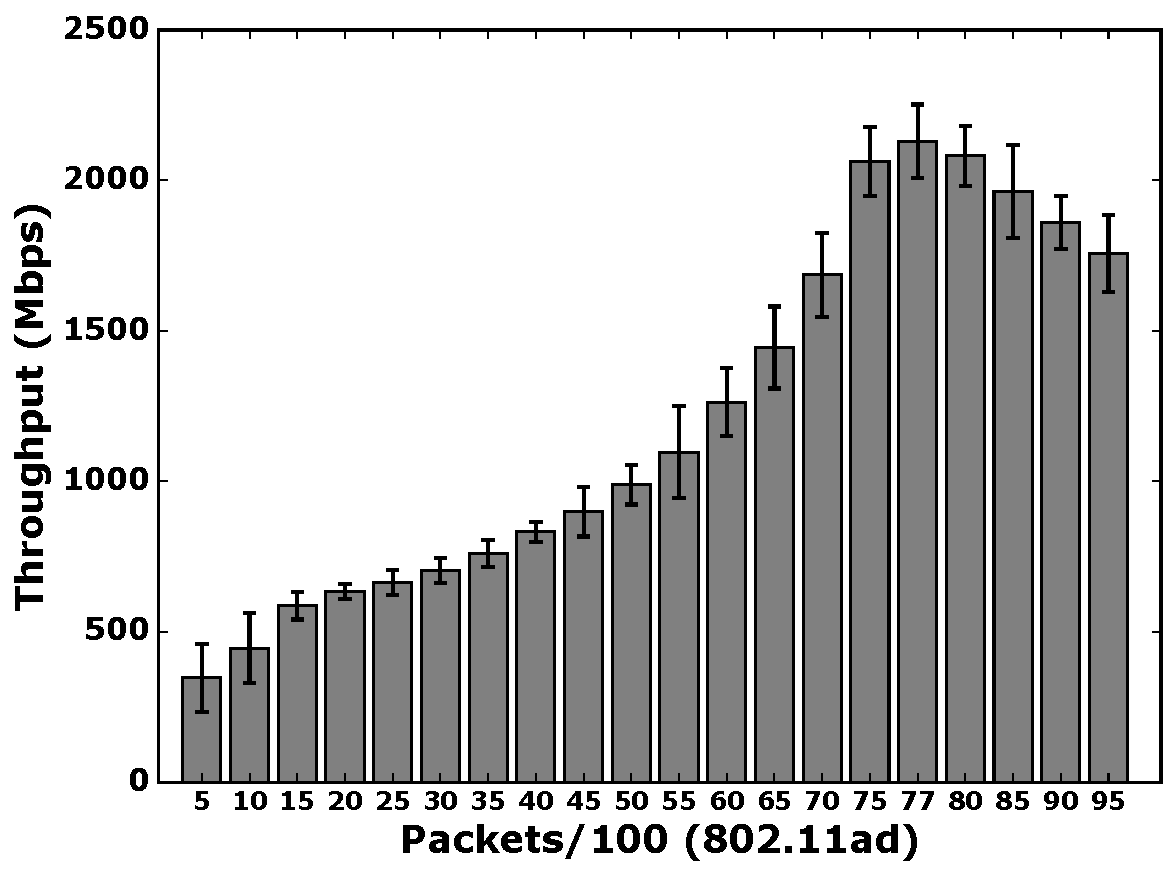
\includegraphics[scale=0.2]{contention/ratio_tput_bar.pdf}
        \label{fig:ratio_tput}
    }\hfill
    \subfigure[Delay (\emph{ofo-queue}): $Pkts_{ad}$] {
        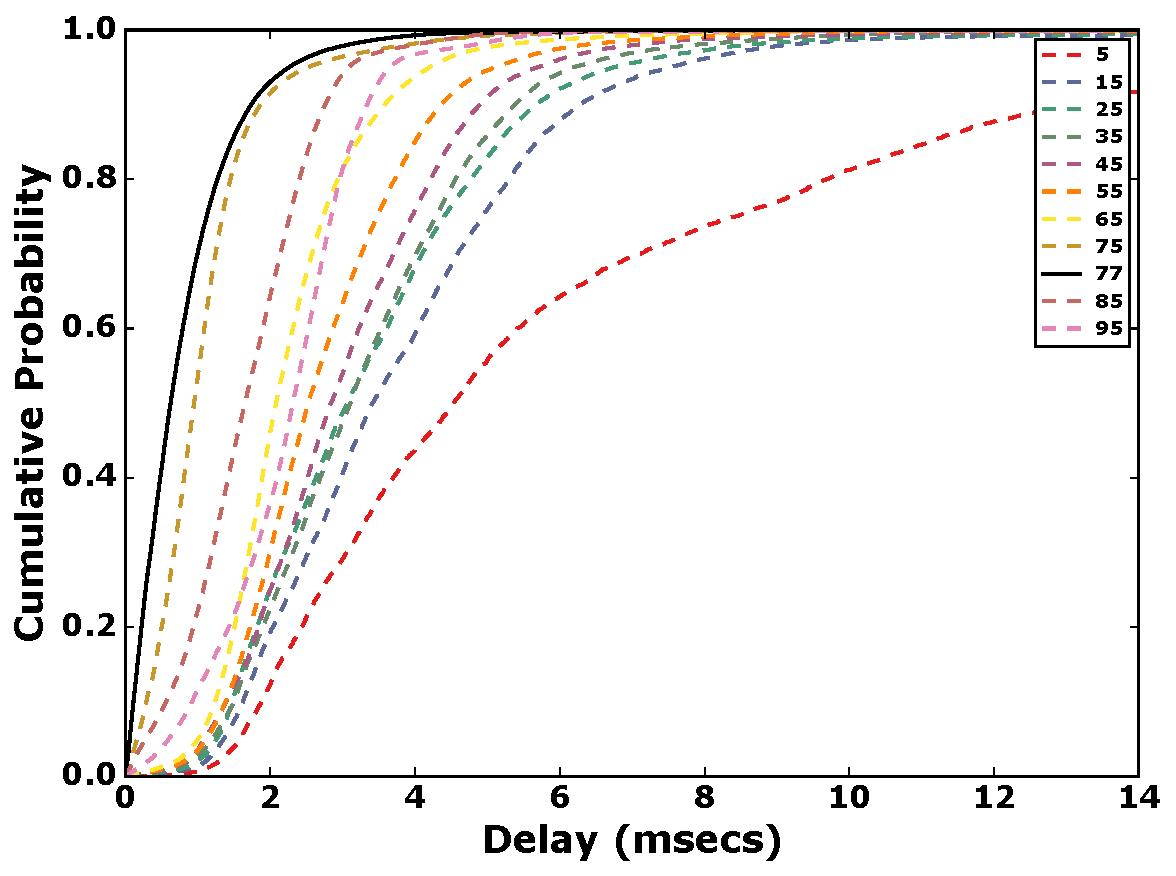
\includegraphics[scale=0.2]{contention/ratio_ofo_delay.pdf}
        \label{fig:ratio_tput_ofo_delay}
    }%\hfill
    %\subfigure[Length of the \emph{ofo-queue} for different $Pkts_{ad}$.] {
    %    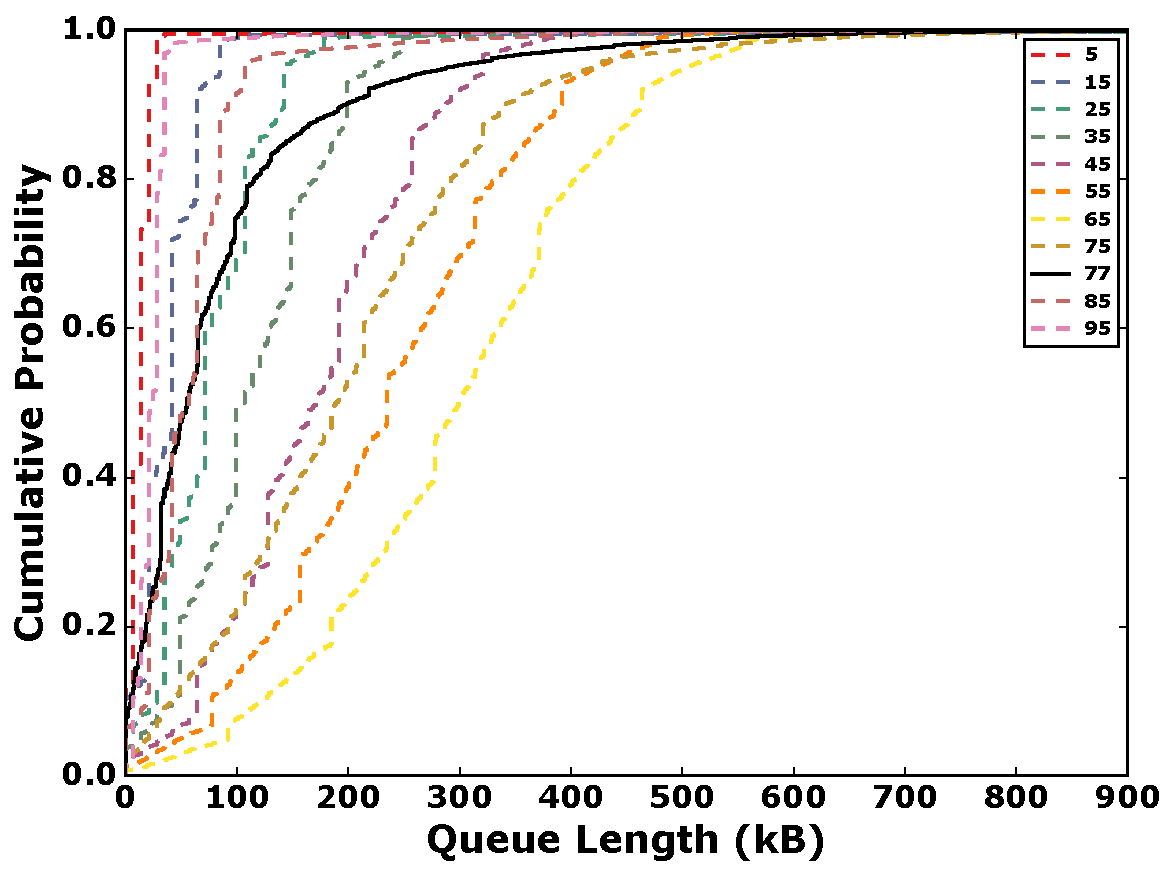
\includegraphics[scale=0.28]{contention/ratio_ofo_q_len.pdf}
    %    \label{fig:ratio_tput_ofo_len}
    %}
    \vspace{-0.2in}
    \caption{Impact of packet scheduling decisions.}
    \vspace{-0.25in}
\end{figure}
Fig.~\ref{fig:ratio_tput} plots the MPTCP throughput against the
number of packets assigned to the 802.11ad subflow ($Pkts_{ad}$) out
of every 100 packets. 
%We vary $Pkts_{ad}$ between 5 to 95 (with a step
%of 5) to cover the entire range of possible assignment ratios. In each
%case, the remaining packets (out of 100) are assigned to the 802.11ac
%subflow ($Pkts_{ac}=100-Pkts_{ad}$).
Maximum throughput of $\sim$2.1 Gbps is achieved with $Pkts_{ad}=77$ and performance worsens as we
move away from this value with the worst throughput of 400 Mbps ($Pkts_{ad}=5$).

We found that the stark difference in performance with different
assignment ratios is a result of the degree to which packets arrive
\textit{out-of-order} in the end-to-end MPTCP flow 
%due tothe specific distribution of traffic among the subflows.
A higher number of out-of-order packets can cause
packets to be buffered in the receiver's \emph{ofo-queue} and in
extreme cases can even result in throttling of the sender because of
limited/no space in the receiver's buffer. In fact, in
Fig.~\ref{fig:ratio_tput_ofo_delay}, which plots the CDF of the delay
experienced by bytes in the \emph{ofo-queue}, we observe that
the $Pkts_{ad}=77$ value (that results in highest throughput) indeed
yields the lowest delay. 
%Moreover, we observe that in general the
%$Pkts_{ad}$ values that result in high delay are the ones that result
%in lower throughput and vice-versa. 
\if 0
We also plot the CDF of the
occupancy of the \emph{ofo-queue} under different $Pkts_{ad}$
values in fig. \ref{fig:ratio_tput_ofo_len}. Here, one might expect to
see a similar behavior as the delay where the queue lengths are smaller
(indicating less out-of-ordering) for packet assignments that yield
higher throughputs. However, under extreme $Pkts_{ad}$ values
(e.g, 5, 95), the traffic distribution is so skewed towards one of
the subflows that almost all the packets flow through one of
the interfaces, thereby significantly reducing the chance of having an
in-sequence packet being delayed over the other interface. As a result
extreme $Pkts_{ad}$ values (5, 95, 15, 85 15), although sub-optimal
throughput-wise, have queue lengths smaller than the one of the $Pkts_{ad}=77$ case.
Excluding the extremes, other $Pkts_{ad}$ values show a general trend of
having larger queues in conjunction with lower throughputs values.
\fi
\\
\noindent\textbf{Throughput-optimal ratio.} $Pkts_{ad}=77$ results in optimal throughput as the
the underlying packet-distribution ratio imposed by this assignment
$Pkts_{ratio}=Pkts_{ac}/Pkts_{ad}=23/77=0.29$ is nearly identical to
the ratio of the actual individual throughputs of the two interfaces
$Tput_{ratio}=Tput_{ac}/Tput_{ad}=500/1600=0.31$. Assigning packets in
this very specific ratio minimizes the chance of packets arriving
out-of-order at the meta-level MPTCP buffers/queues. 
\if 0
Note that
although in-order delivery of packets within a subflow (intra-subflow)
is guaranteed because of single path TCP (SPTCP) operation at the subflow level,
global in-order delivery among all subflows (inter-flow) needs
to be achieved through re-ordering at the meta-level.
\fi
